\documentclass{beamer}
\mode<presentation>

\usepackage{graphicx}

\usetheme{Singapore} % Dresden?
\title{A Simple Laboratory Environment \\for Real-World Offensive Security Education}
\author{Maxim Timchenko \and David Starobinski}
\institute{Electrical and Computer Engineering Department\\Boston University}
\date{SIGCSE'15, March 7, 2015}
\begin{document}
	\begin{frame}
		\titlepage
	\end{frame}
	
	\section{Motivation}
	\subsection{Goal}
	
	\begin{frame}{Goals for a Laboratory Environment}
		\begin{center}
    		\begin{columns}[t]
		\begin{column}{0.1\textwidth}
		~
		\end{column}
     		\begin{column}{0.4\textwidth}
            		Must Have\\~
            		\begin{itemize}
            			\item Security\\~
            			\item Isolation
            		\end{itemize}		
      		\end{column}
    
    		\begin{column}{0.4\textwidth}
            		Stretch Goals\\~
            		\begin{itemize}
            			\item Redundancy\\~
            			\item Persistence
            		\end{itemize}		
      		\end{column}
    		\end{columns}			
		\end{center}
	\end{frame}

	\begin{frame}{``Real-world'' and ``Offensive''}
		\begin{itemize}
			\item Use the tools commonly used within the industry	
%			\begin{itemize}			
%				\item Practical experience
%				\item Reuse
%				\item Plenty of reference information
%			\end{itemize}				
			\item Discuss actual exploits, demonstrate issues vividly
			\begin{itemize}
				\item Metasploit modules
				\item Social engineering
			\end{itemize}
			\item Cover current events (e.g. 2014: Shellshock, Heartbleed)
			\item Attacker mindset vs. developer mindset
		\end{itemize}		
		~
		\begin{center}
			
\includegraphics[width=0.2\textwidth]{heartbleed.png}
		\end{center}
	\end{frame}

	\begin{frame}{``Simple''}
		\begin{itemize}
			\item Simple to install and use
			\item Reuse available parts
			\item This is an {\em introductory} course
		\end{itemize}	
	\end{frame}
		
%	\begin{frame}{``Offensive''}
%		\begin{itemize}
%			\item Attacker mindset vs. developer mindset
%			\begin{itemize}
%				\item ``How can I make this do something else''?
%				\item Low-level, in-depth understanding
%				\item Challenge bad assumptions
%			\end{itemize}
%			\vfill
%			\item Both sides of the coin
%			\begin{itemize}			
%				\item Looking only at defense makes attacks ``abstract''
%				\item Immediate reaction to trying attacks out
%				\item Then, discuss how to defend
%			\end{itemize}		
%			\vfill		
%			\item Students love it!
%		\end{itemize}
%	\end{frame}

	\section{Environment}	
	\subsection{dummy-name}
	
	\begin{frame}{Environments}
		Local isolated network containing actual hardware
		\vfill
		\begin{columns}
 		\begin{column}{0.5\textwidth}
    			\begin{itemize}
        				\item Expensive
        				\item Limited flexibility
        				\item Limited sharing
    			\end{itemize}
  		\end{column}

		\begin{column}{0.5\textwidth}
     			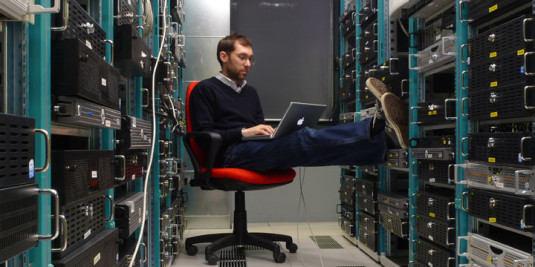
\includegraphics[width=\textwidth]{env-datacenter_rizzi.jpg}
			
			{\tiny Photo: Leonardo Rizzi, Flickr, Creative Commons}
  		\end{column}
		\end{columns}
	\end{frame}
	
	\begin{frame}{Environment Virtualization}
		\begin{block}{Centralized On Premises}
			\only<1>{
            		\begin{columns}
             		\begin{column}{0.5\textwidth}
                			\begin{itemize}
                    			\item Set-up and maintenance
                    			\item Limited scaling
					\item Example: Tele-Lab [10]
                			\end{itemize}
              		\end{column}
            
            		\begin{column}{0.5\textwidth}
				\begin{center}
                 		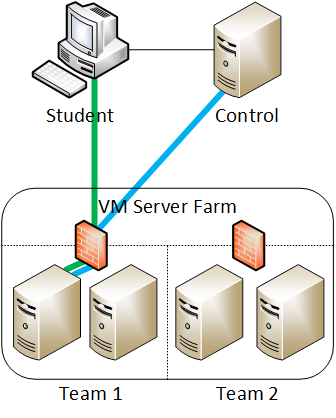
\includegraphics[width=0.6\textwidth]{centralized-virt.png}
				\end{center}
              		\end{column}
            		\end{columns}
			}
		\end{block}
		\begin{block}{Cloud}
			\only<2>{
            		\begin{columns}
             		\begin{column}{0.5\textwidth}
                			\begin{itemize}
					\item Complicated architecture
                    			\item Expensive scaling
                    			\item Potentially, worst responsiveness\\(traffic and delay)
					\item Example: Salah [6] on AWS
                			\end{itemize}
              		\end{column}
            
            		\begin{column}{0.5\textwidth}
						\begin{center}
                 		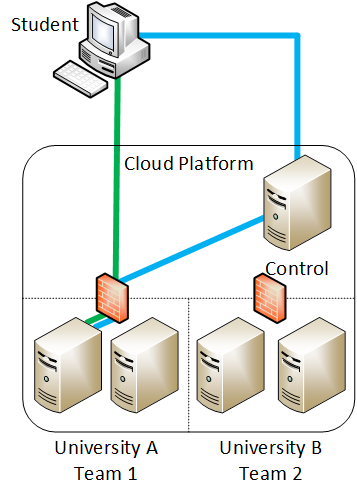
\includegraphics[width=0.6\textwidth]{cloud-virt.png}
				\end{center}
              		\end{column}
            		\end{columns}		
			}
		\end{block}
		\begin{block}{Local}
			\only<3>{
            		\begin{columns}
             		\begin{column}{0.5\textwidth}
                			\begin{itemize}
                    			\item Easy set-up
                    			\item No scaling issues
                    			\item Best responsiveness
					\item Example: SEED [2] on VMWare/VirtualBox
                			\end{itemize}
              		\end{column}
            
            		\begin{column}{0.5\textwidth}
				\begin{center}
                 		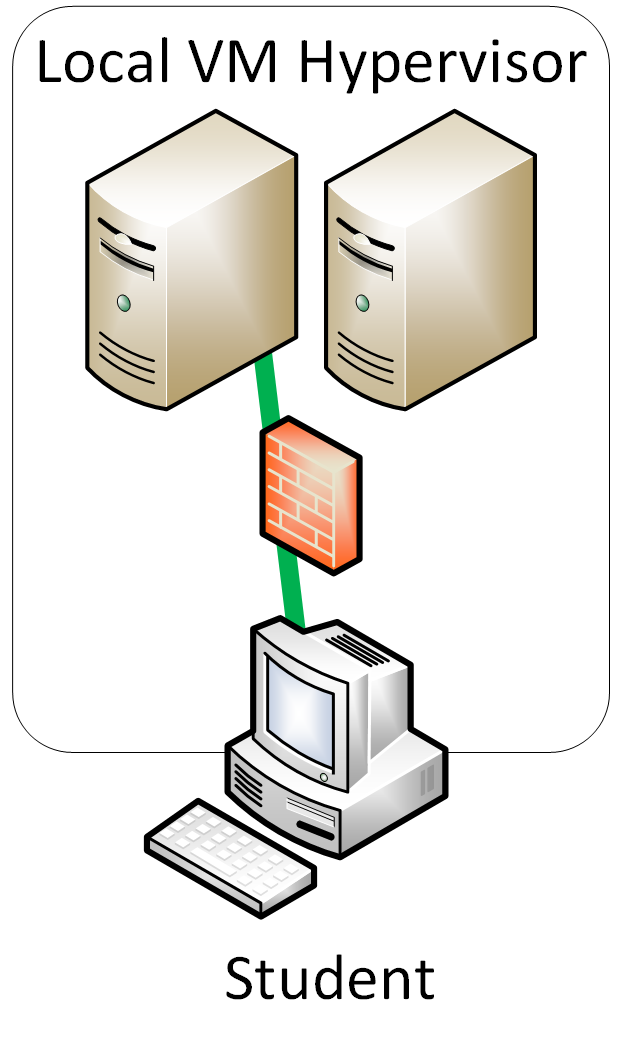
\includegraphics[width=0.4\textwidth]{local-virt.png}
				\end{center}
              		\end{column}
            		\end{columns}		
			}	
		\end{block}		
	\end{frame}	

	\begin{frame}{Detailed Environment Architecture}
		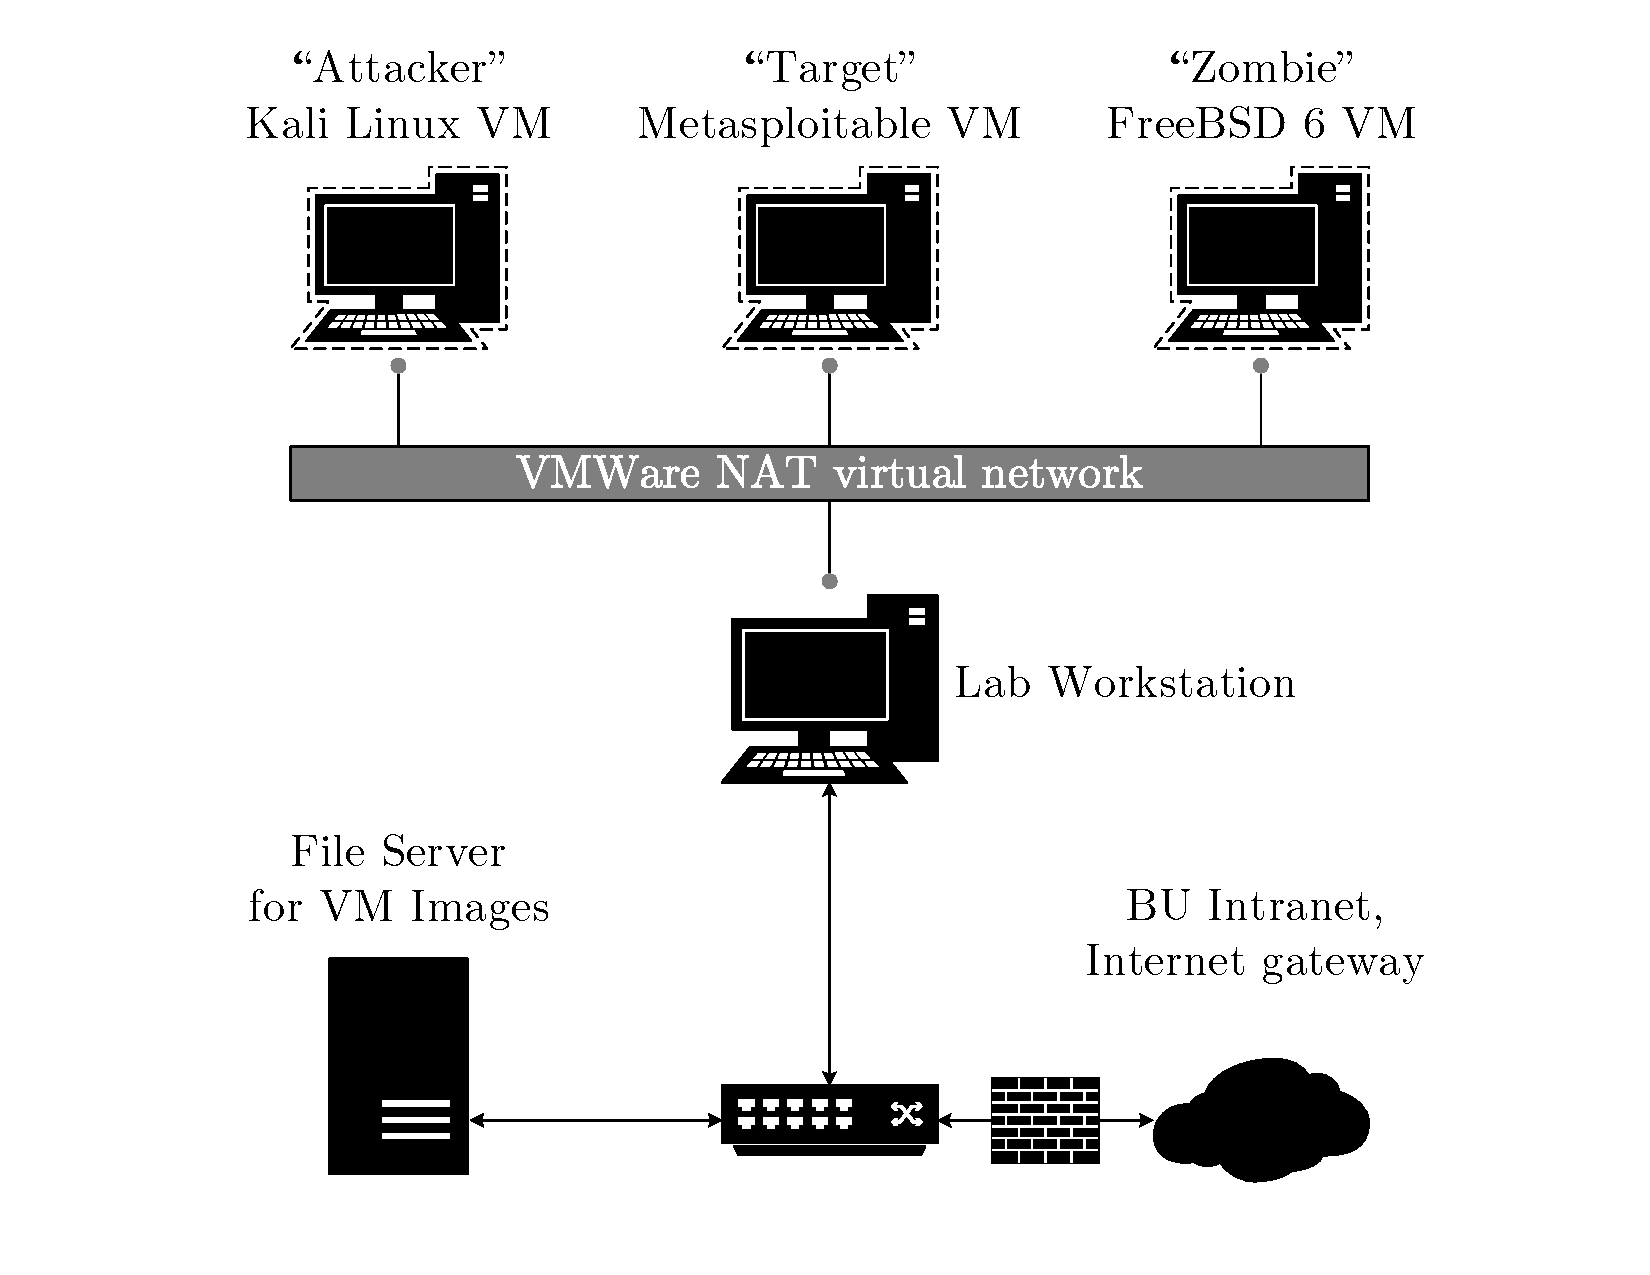
\includegraphics[page=1,width=\textwidth]{../paper/ec521_hostmap.pdf}
	\end{frame}

	\begin{frame}{VM Image Sets}
		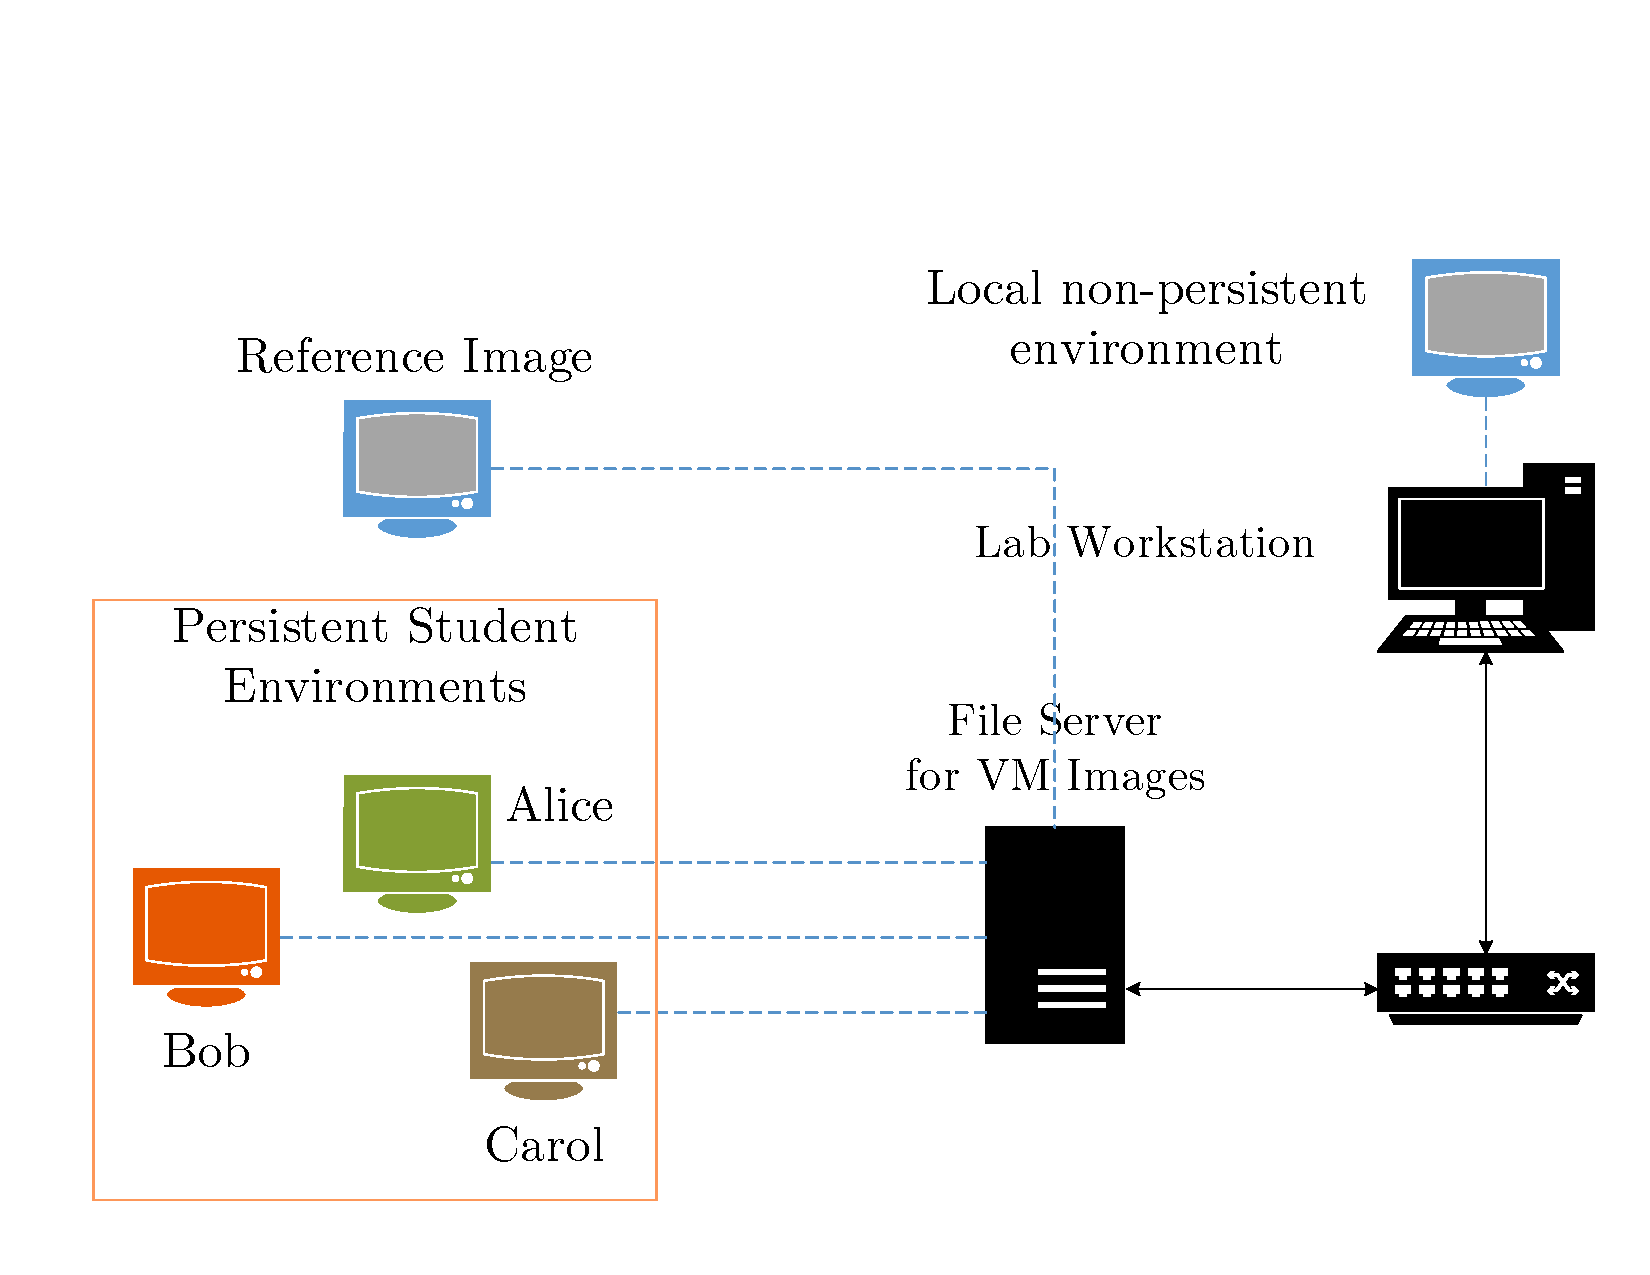
\includegraphics[page=1,width=\textwidth,clip=true, trim=0 0 0 1in]{vm-image-sets.pdf}
	\end{frame}
	
	\begin{frame}{The Attacker - Kali Linux}
            		\begin{columns}
             		\begin{column}{0.5\textwidth}
                			\begin{itemize}
                    			\item Pentesting and Auditing
                    			\item Based on Debian Wheezy
                    			\item Hundreds of tools
					\item Top 10: Aircrack, Burp Suite, Hydra, John, Maltego, Metasploit, NMAP, ZAP, SQLmap, Wireshark
					\item Maintained by {\em Offensive Security}
                			\end{itemize}
              		\end{column}
            
            		\begin{column}{0.5\textwidth}
				\begin{center}
                 		
\includegraphics[width=\textwidth]{kali-bg.png}
				\end{center}
              		\end{column}
            		\end{columns}				
	\end{frame}
	
	\begin{frame}{The Target - Metasploitable 2}
            		\begin{columns}
             		\begin{column}{0.5\textwidth}
                			\begin{itemize}
                    			\item Intentionally Vulnerable VM
                    			\item Based on Ubuntu
                    			\item Many vulnerabilities of various obviousness
					\item Two intentionally vulnerable web applications (DWVA, Mutillidae)
%					\item Mutilidae covers all the top ten OWASP vulnerabilities and more
					\item No GUI
                			\end{itemize}
              		\end{column}
            
            		\begin{column}{0.5\textwidth}
				\begin{center}
                 		\includegraphics[width=\textwidth]{metasploitable2_booted.png}
				\end{center}
              		\end{column}
            		\end{columns}				
	\end{frame}	

	\begin{frame}{Resource Requirements}
		\includegraphics[page=2,width=\textwidth, clip=true, trim=0.5in 6in 1in 0.5in]{Resources.pdf}
	\end{frame}
		
	\begin{frame}{Studying Cybersecurity Anywhere}
		\begin{center}
		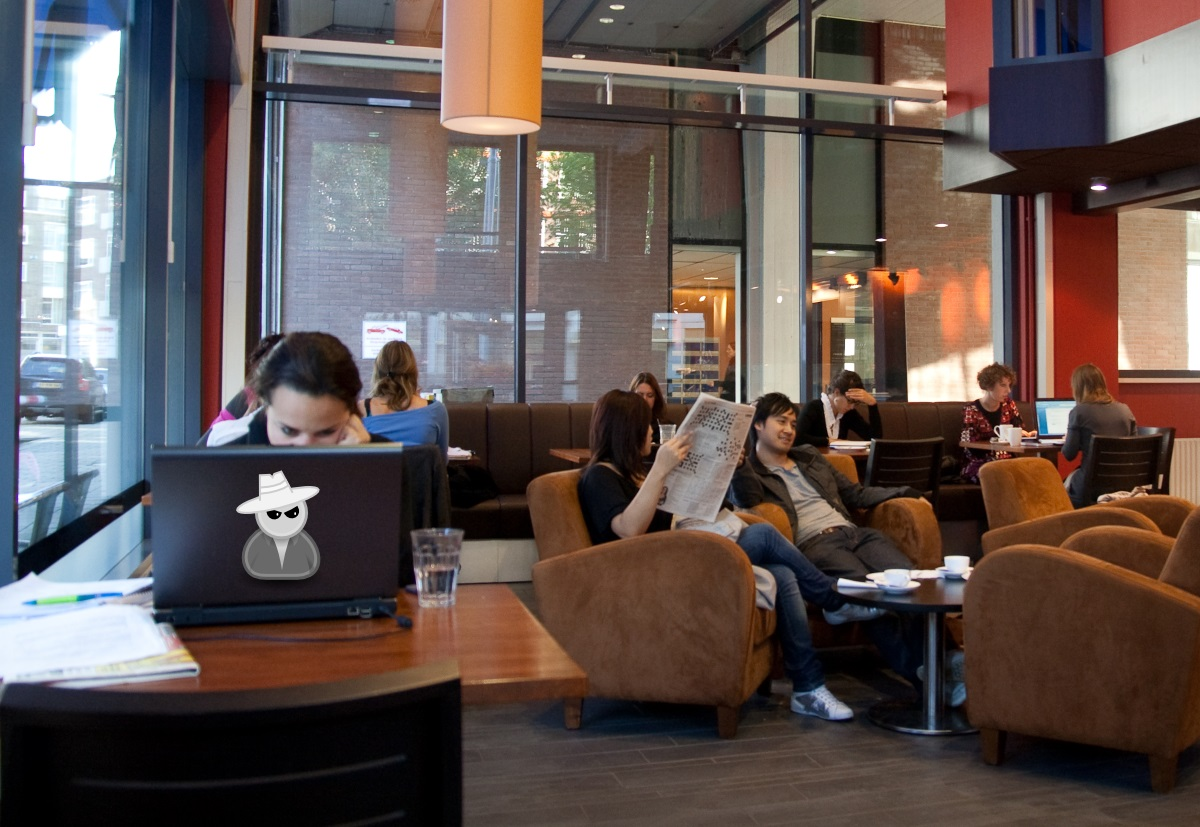
\includegraphics[width=0.8\textwidth]{coffeeshop_whitehat.jpg}
		
		{\tiny Photo: Alper Cugun, Flickr, CC-BY 2.0 | Whitehat Icon: Open Security Architecture, CC-BY-SA}
		\end{center}
	\end{frame}
	
	\section{Labs}
	\subsection{dummy-name}
	\begin{frame}{Existing Lab Sets}
		\begin{columns}
             		\begin{column}{0.5\textwidth}
				\begin{center}
					
\includegraphics[width=0.4\textwidth]{seed-labs-logo.png} \\
	                			The SEED Project [2]
				\end{center}
              		\end{column}
			\pause		
            		\begin{column}{0.5\textwidth}			
				\begin{center}
					
\includegraphics[width=0.8\textwidth]{owasp-logo.jpg} \\
					
\includegraphics[width=\textwidth]{hackademic-logo.png}
					
					OWASP Hackademic [5]
				\end{center}
              		\end{column}
		\end{columns}			
		\vfill
		\begin{columns}
            		\begin{column}{0.5\textwidth}
            		\pause	
			\begin{center}	
			Many papers containing\\one or two labs each
			\end{center}
             		\end{column}
			\pause
            		\begin{column}{0.5\textwidth}				
			\begin{center}
			Internet tutorials, e.g. ``How to use Metasploit to hack X''
			\end{center}
              		\end{column}
		\end{columns}	
	\end{frame}
	
	\begin{frame}{Lab Topics and Dependencies}
		\begin{center}
		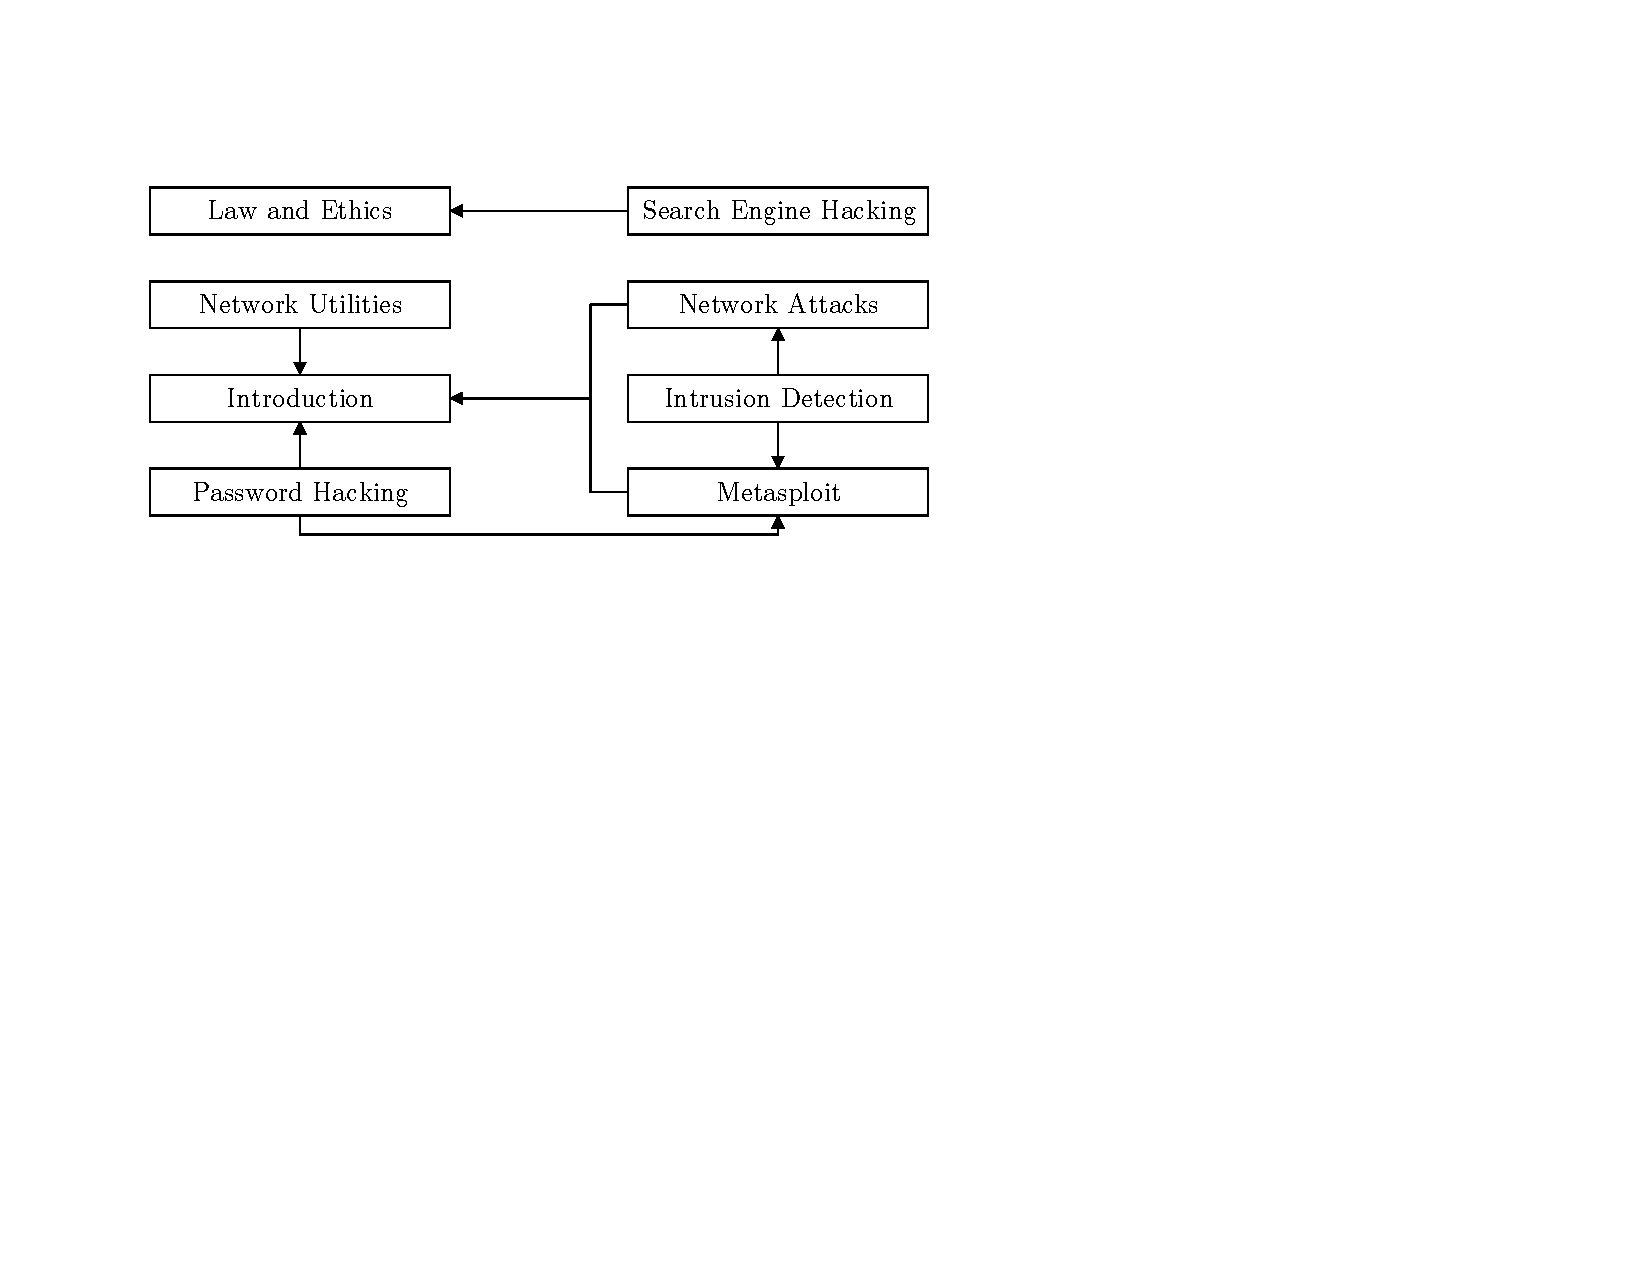
\includegraphics[width=\textwidth,clip=true, trim=0.85in 4.75in 4.5in 1.2in]{../paper/dependencies-between-labs.pdf}
		\end{center}		
	\end{frame}	
	
	\begin{frame}{Network Attacks Lab}
            		\begin{columns}
             		\begin{column}{0.5\textwidth}
                			\begin{itemize}
                    			\item Zombie scan with {\texttt nmap}
                    			\item ARP Poisoning
					\item DNS resolving and caching
                    			\item DNS Poisoning
					\item Example: poison Metasploitable's DNS and replace one website with another
                			\end{itemize}
              		\end{column}
            
            		\begin{column}{0.5\textwidth}
				\begin{center}
                 		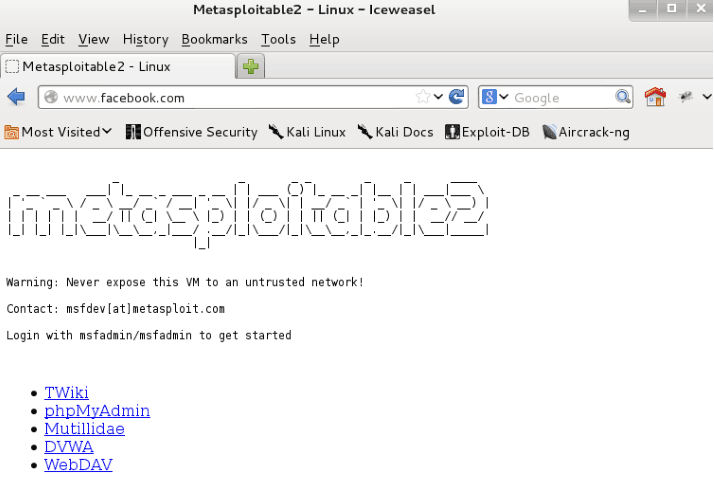
\includegraphics[width=\textwidth]{../labs/network-attacks/the-new-facebook.png}
				\end{center}
              		\end{column}
            		\end{columns}				
	\end{frame}		
	
	\begin{frame}{Sample Page}
		\begin{center}
		\fbox{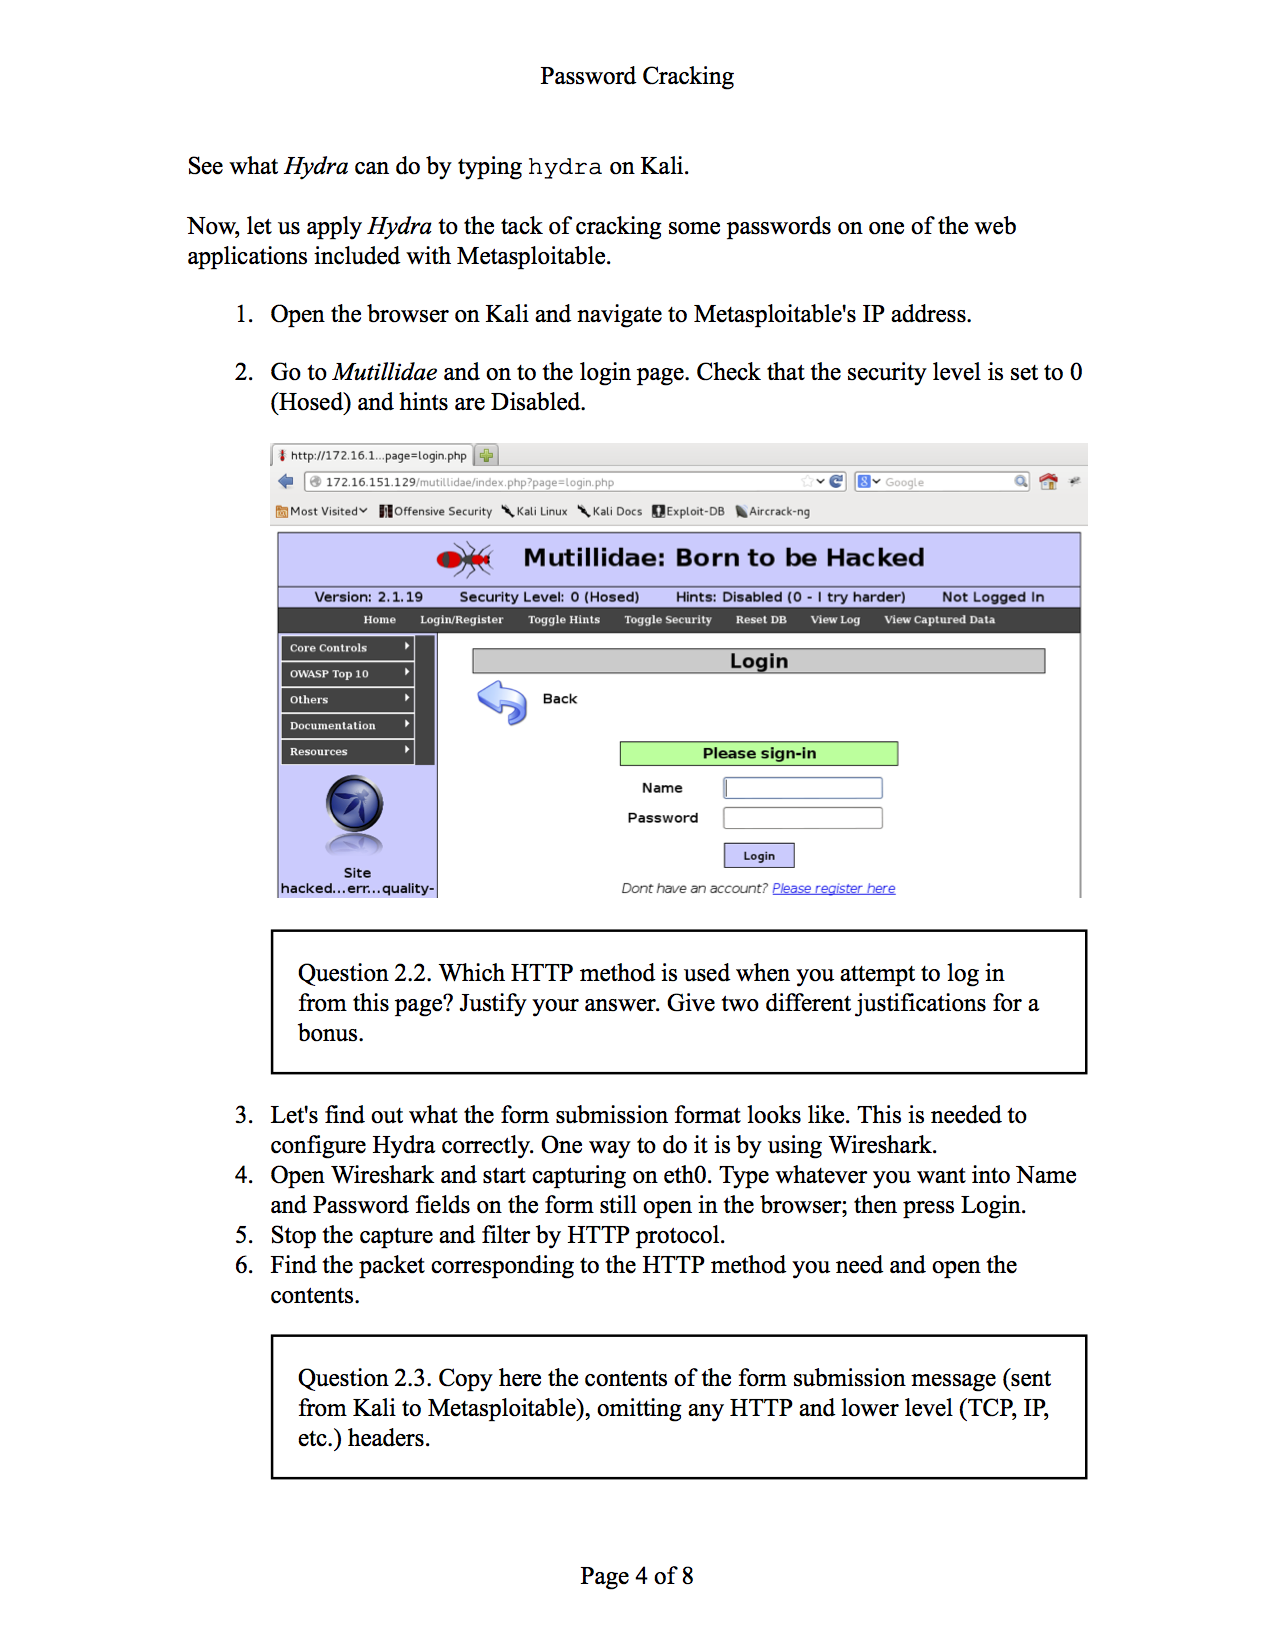
\includegraphics[width=0.5\textwidth]{lab7-sample-page.png}}
		\end{center}		
	\end{frame}	
	
	\begin{frame}{Sample Solution Page}
		\begin{center}
		\fbox{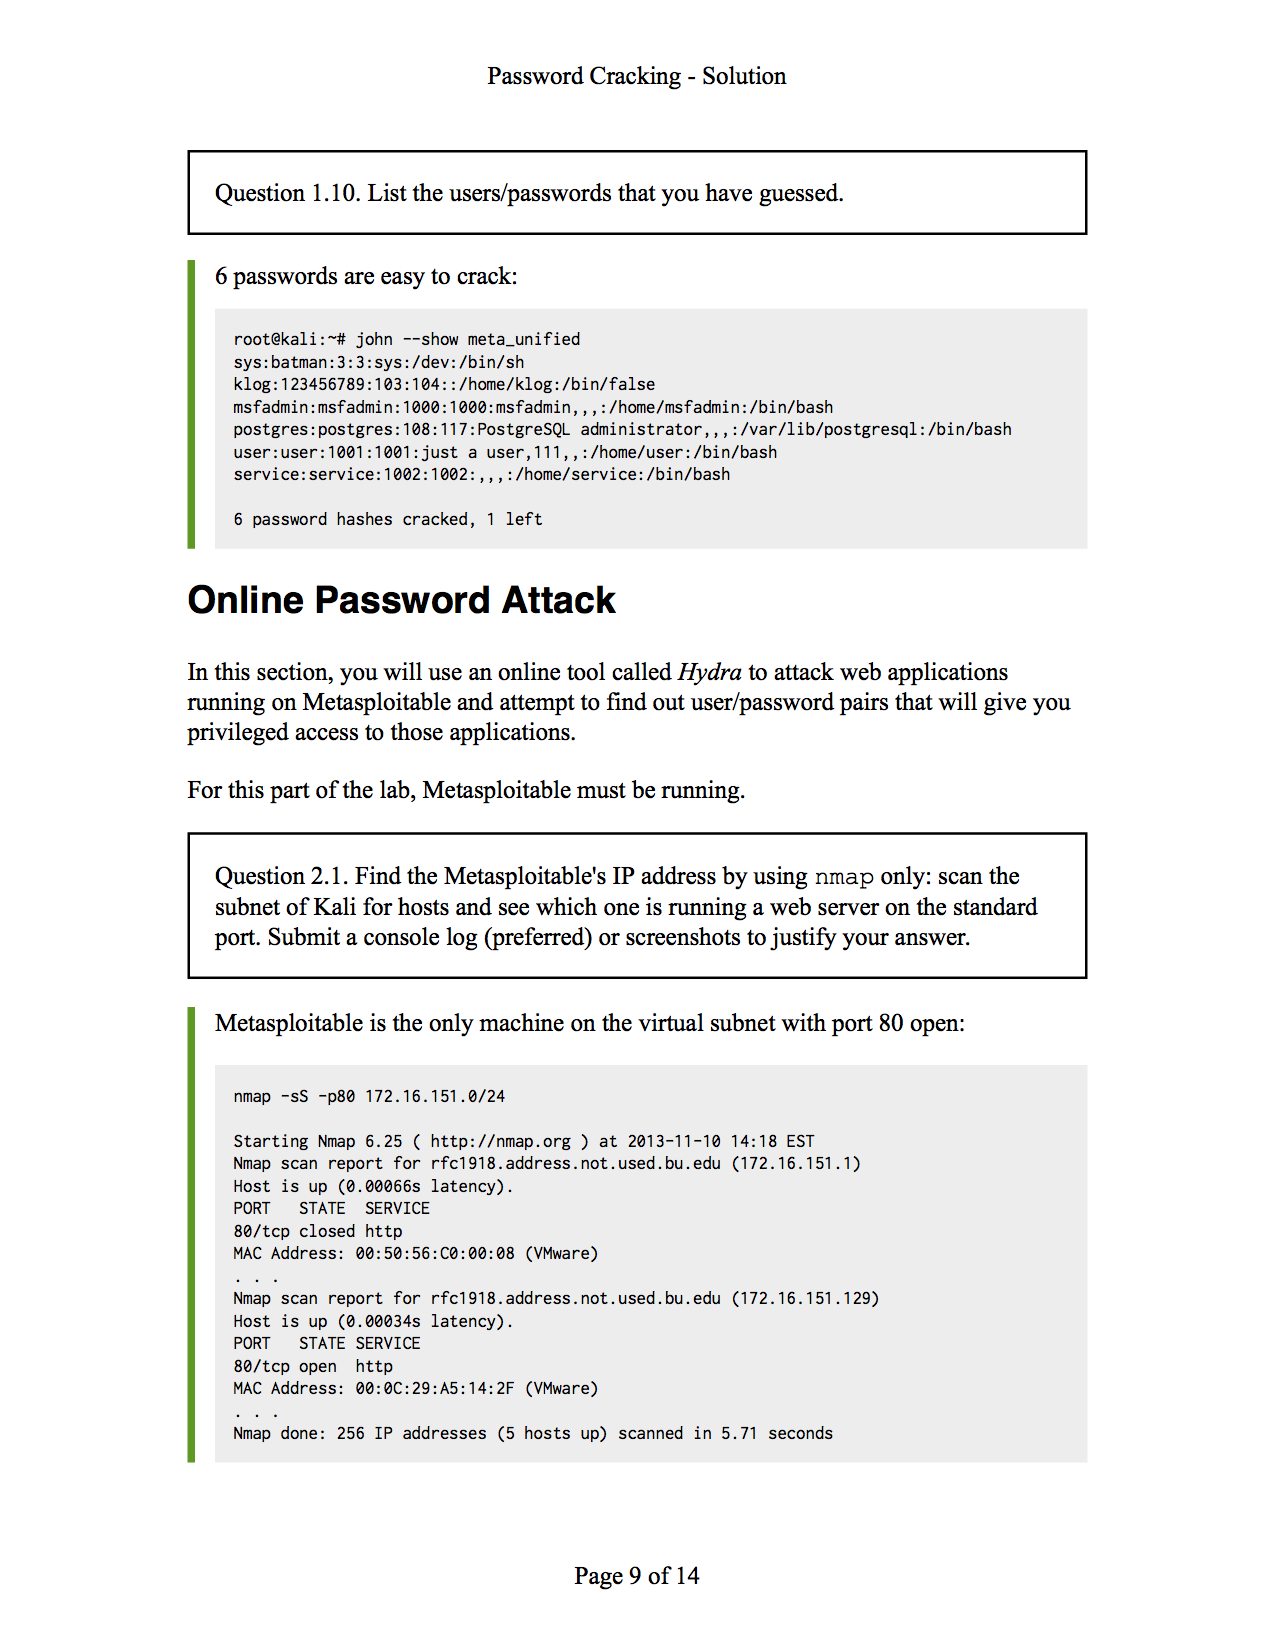
\includegraphics[width=0.5\textwidth]{lab7-solution-page.png}}
		\end{center}		
	\end{frame}
	
	\begin{frame}{Production Workflow (PDF)}
		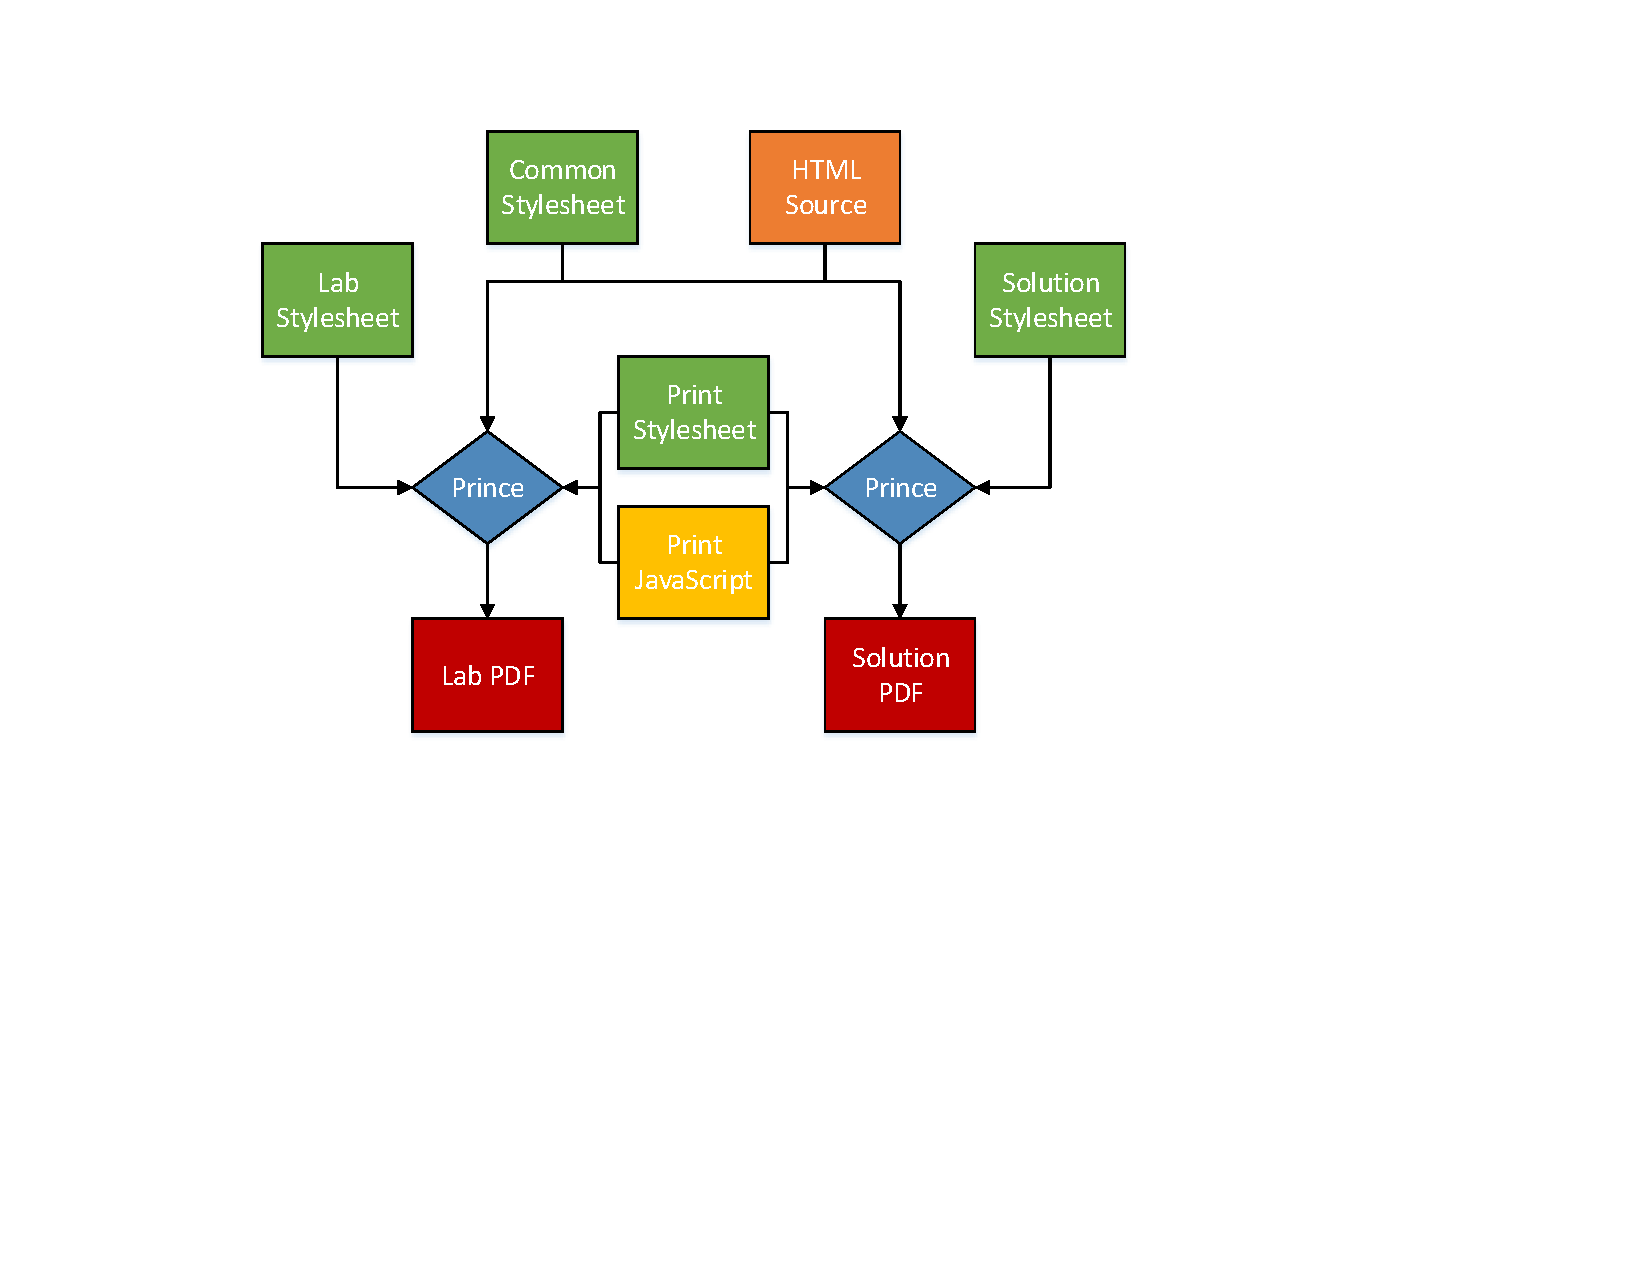
\includegraphics[width=\textwidth, clip=true, trim=1.3in 3in 3in 0.5in]{workflow.pdf}
	\end{frame}			

	\begin{frame}{Production Workflow (HTML)}
		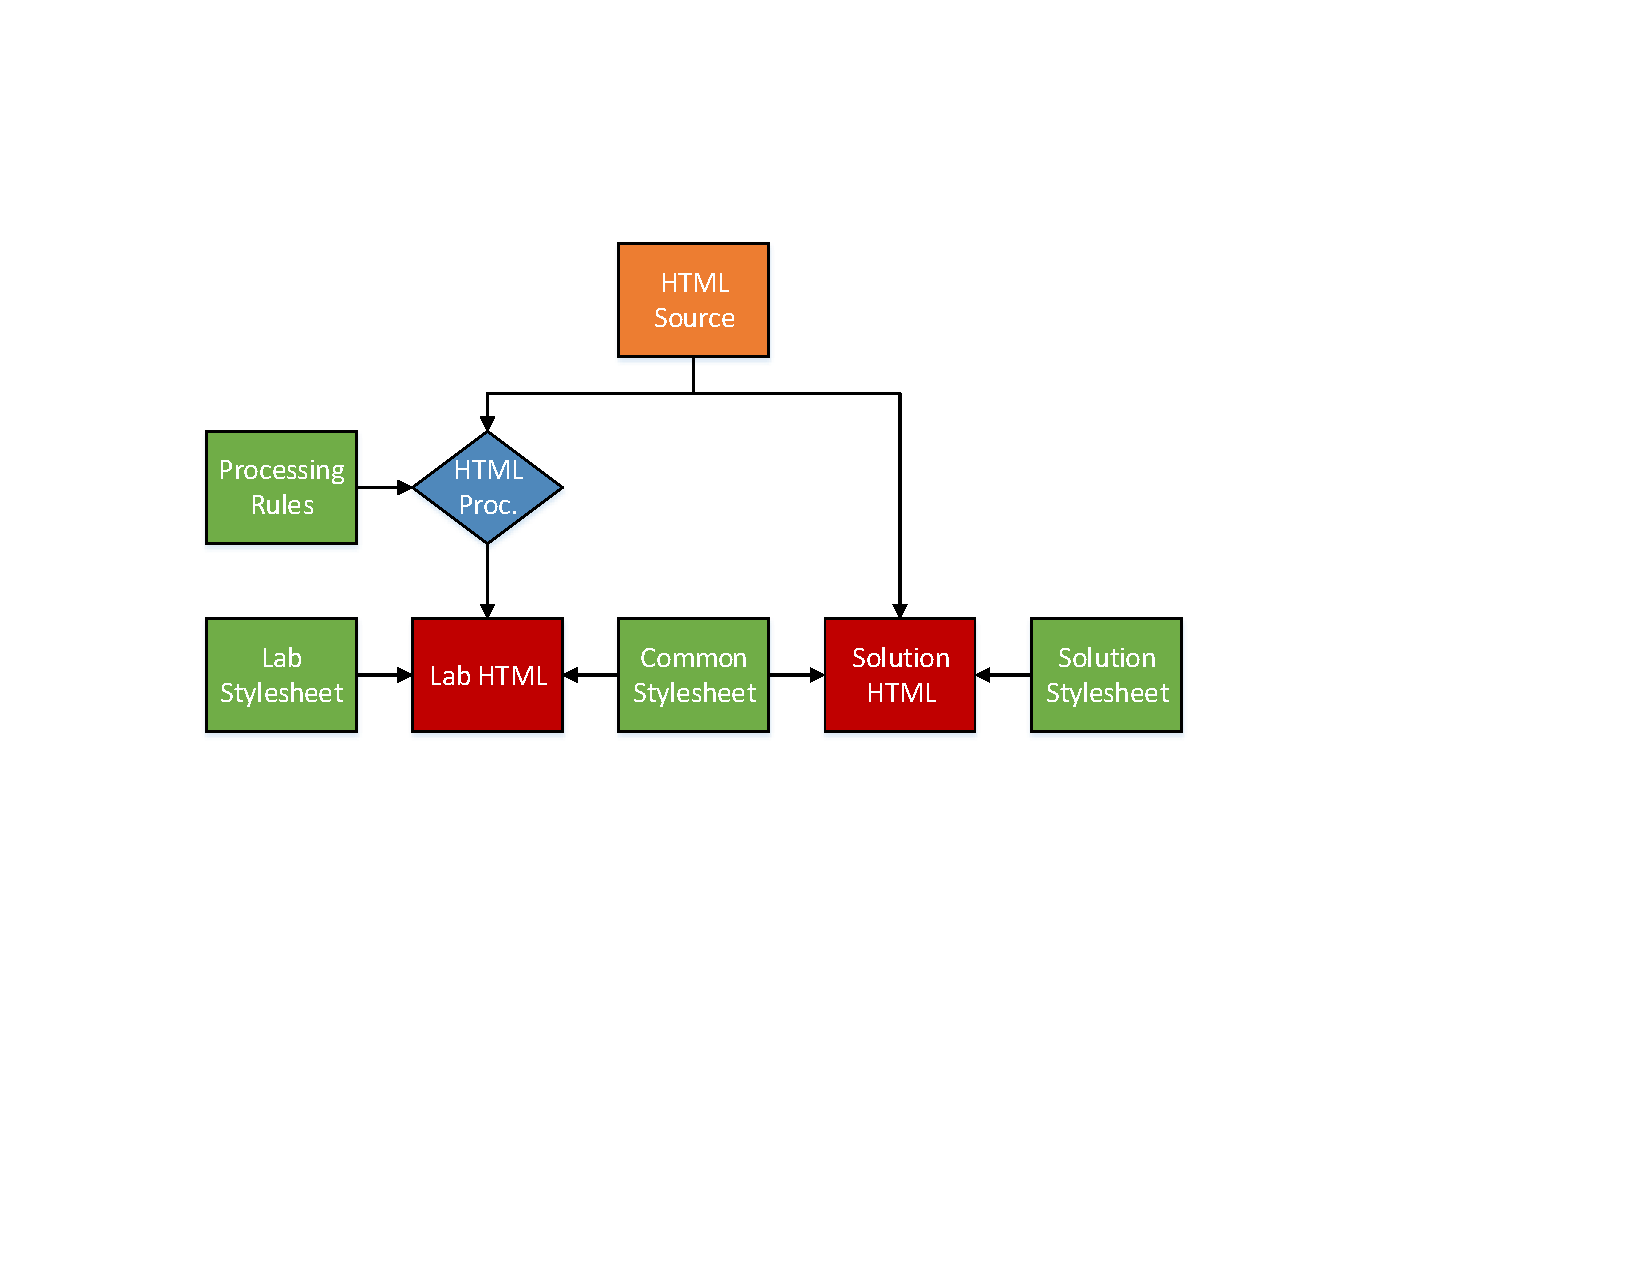
\includegraphics[width=\textwidth, clip=true, trim=1.3in 3in 3in 0.5in]{online-workflow.pdf}
	\end{frame}	
		
	\section{Future Work}
	\subsection{dummy-name}
				
	\begin{frame}{Directons for Future Work}
		\begin{itemize}	
			\item Updates to Metasploitable
			\item Easier modifications to Metasploitable
			\item Adding other OS images and platforms
			\item Adding network device simulation\\(routers, peripherals. SDN?)
			\item Automated grading
		\end{itemize}
	\end{frame}

	\section{Summary}
	\subsection{dummy-name}	
	\begin{frame}{Summary}
		\begin{itemize}
			\item	A virtual-machine based environment for teaching practical cybersecurity
%			\begin{itemize}			
%				\item Requires no additional infrastructure
%				\item Runs well on current hardware, including laptops
%			\end{itemize}	
			\pause			
			\item A set of structured labs based on the environment
%			\begin{itemize}			
%				\item A choice of topics for an introductory course
%				\item Structured, guided assignments
%				\item Try to build each lab on previous ones to reinforce
%			\end{itemize}	
			\pause
			\item Directions for future work
%			\begin{itemize}			
%				\item Automated grading a prerequisite for scaling
%				\item How to maintain and extend the VMs going forward?
%				\item Add architectures (mobile/IoT) and network devices (SDN)
%			\end{itemize}								
		\end{itemize}
	\end{frame}
	
	\begin{frame}{Thank you for your attention!}
		The sources for this talk and several of the labs can be found in our GitHub repository:
		\vfill
		\begin{center}
		\url{https://github.com/maxvt/cyberlabs}
		\end{center}
		\vfill
		Contact the authors at:
		\begin{itemize}
			\item \texttt{staro@bu.edu}
			\item \texttt{maxvt@bu.edu}, 
\includegraphics[width=9pt]{Twitter_bird_logo_2012.png}\hspace{0.2em}\texttt{@maxvt}
			\item \url{http://nislab.bu.edu/}
		\end{itemize}	
	\end{frame}
\end{document}